 \documentclass[12pt,openright,twoside]{report}
 \usepackage{etoolbox}
 \makeatletter
\newif\if@abstractmode

\renewenvironment{titlepage}
{
  \if@twocolumn
  \@restonecoltrue\onecolumn
  \else
  \@restonecolfalse\newpage
  \fi
  \if@abstractmode
  \thispagestyle{plain}%
  \stepcounter{page}%
  \else
  \thispagestyle{empty}%
  \setcounter{page}\@ne%
  \fi
}%
{\if@restonecol\twocolumn \else \newpage \fi
  \if@twoside\else
  \if@abstractmode
  \else
  \setcounter{page}\@ne%
  \fi
  \fi
}

\AtBeginEnvironment{abstract}{%
  \@abstractmodetrue%
}


\makeatother
\usepackage[english]{babel}
\usepackage[utf8x]{inputenc}
\usepackage[twoside,paper=a4paper, top=1in,bottom=1.5in,inner=1in,outer=1.5in]{geometry}

\newcommand{\me}{\mathrm{e}}
\usepackage{amsmath}
\usepackage{tabularx}
\usepackage{setspace}
\usepackage{lscape}
%\usepackage{natbib}
%\usepackage[backend=biber]{biblatex}
\usepackage{multicol}
\usepackage{multirow}
\usepackage{ragged2e}
\usepackage{graphicx}
\usepackage{adjustbox}
\usepackage{hyperref}
\usepackage[square,sort,comma,numbers]{natbib}
\usepackage[toc,page]{appendix}
\usepackage[colorinlistoftodos]{todonotes}
%\oddsidemargin .5cm
%\evensidemargin .5cm



\begin{document}

\begin{titlepage}
\newgeometry{top=0.6in,bottom=0.5in,right=1in,left=1.5in}
\vspace{-500cm}
%\newcommand{\HRule}{\rule{\linewidth}{0.5mm}} % Defines a new command for the horizontal lines, change thickness here

\center % Center everything on the page
 
%----------------------------------------------------------------------------------------
%	HEADING SECTIONS
%----------------------------------------------------------------------------------------
.\\[0.6cm]
\textsc{\Large \textbf{An Internship Report\\[0.80cm]on}}\\[0.80cm] % Major heading
% Name of your university/college
\textsc{\Large \textbf{Write the Title here}}\\[0.80cm] % Title of Project

{ \it in partial fulfillment for the award of the degree \\[0.80cm]of \\[0.80cm]

\large{BACHELOR OF TECHNOLOGY (B.TECH)\\[0.8cm]}{IN\\[0.8cm]ELECTRICAL ENGINEERING}\\[1.6cm] Submitted by}\\[0.8cm]
\
\textsc{\textbf{Amit Katare (0901EE171019)}} \\[1.60cm]

%----------------------------------------------------------------------------------------
%	TITLE SECTION
%----------------------------------------------------------------------------------------


\includegraphics[width=3.5cm]{images.jpg}\\[0.80cm]
 
%----------------------------------------------------------------------------------------
%	AUTHOR SECTION
%----------------------------------------------------------------------------------------
\textsc{\textbf{MADHAV INSTITUTE OF TECHNOLOGY $\&$ SCIENCE}}\\[0.15cm]\textbf{Gwalior (M.P.) - 474001}\\[0.15cm] \footnotesize{\it{\textbf{(A Govt. Aided UGC Autonomous $\&$ NAAC Accredited Institute Affiliated to RGPV, Bhopal)}}} \\[0.15cm] \textbf{JUNE, 2021}
\end{titlepage}
\clearpage

\newpage
\pagenumbering{roman}
%**************************Start of Certificate
%\chapter*{Certifi}
\newgeometry{top=0.8in,bottom=1in,right=0.8in,left=1.3in}
\vspace*{-0.3cm}

\begin{center}  {\normalsize \bf DECLARATION}\\
\end{center}
%\begin{center}  {\small{\bf  DEPARTMENT OF ELECTRICAL ENGINEERING}}\vspace{0.1cm}\end{center}

\justify
\doublespace
I/We hereby declare that the internship report titled \textbf{"Analysis of Speed Control of Brushless Direct Current Motor"} submitted for the award of \textbf{Bachelor of Technology} degree in \textbf{Electrical Engineering} is my original work and the report has not been submitted elsewhere for the award of any other degree, diploma, fellowship or any other similar titles. 
\\[0.8cm]
\begin{minipage}{1\textwidth}
\begin{flushright} \normalsize\\

Amit Katare (0901EE171019)\\[0cm]
\end{flushright}
\end{minipage}\\[0.4cm]
\begin{minipage}{1\textwidth}
\begin{flushleft} \normalsize\\
Place:                                                            Gwalior\\
Date: 16/06/2021
\end{flushleft}
\end{minipage}\\[0.4cm]
\begin{minipage}{1\textwidth}
\begin{flushright} \normalsize\\
\hline
\end{flushright}
\end{minipage}\\[0.4cm]
\begin{minipage}{1\textwidth}
\begin{flushleft} 
This is to certify that the above statement made by the candidate’s is correct to my knowledge and belief.
\end{flushleft}
\end{minipage}\\[1.2cm]
\begin{minipage}{0.5\textwidth}
\begin{flushleft} \normalsize
\textbf{Approved By}\\[1.5cm]
\textbf{Dr. Sulochana Wadhwani }\\[0cm]
Professor $\&$ Head\\[0cm]
Dept. of EE\\[0cm]
MITS, Gwalior
\end{flushleft}
\end{minipage}
\begin{minipage}{0.5\textwidth}
\begin{flushright} \normalsize
\textbf{Guided By}\\[1.5cm]
\textbf{Dr.  }\\[0cm]
(Professor) \\[0cm]
Dept. of EE\\[0cm]
MITS, Gwalior
\end{flushright}
\end{minipage}\\[1.5cm]
\begin{minipage}{1\textwidth}
\begin{flushright} \normalsize
\textbf{Dr. }\\[0cm]
(Assistant Professor) \\[0cm]
Dept. of EE\\[0cm]
MITS, Gwalior
\end{flushright}
\end{minipage}\\[0.8cm]
\begin{minipage}{1\textwidth}
\begin{flushright} \normalsize

\end{flushright}
\end{minipage}
%***************\End of certificate
\newpage
%************************ Start of Acknowledgement
%\thispagestyle{empty}
\newgeometry{top=1in,bottom=1in,inner=0.8in,outer=1.3in}
\vspace*{-0.3cm}
\begin{center}
\textsc{\Large \bf Acknowledgements}
\end{center}\vspace{1cm}
\justify
\doublespace
We take enormous happiness in conveying our deep feeling of appreciation to our respected institute MADHAV INSTITUTE OF TECHNOLOGY & SCIENCE, GWALIOR (M.P) for giving us the chance to complete our project.






%************************ End of Acknowledgement
\newpage
\newgeometry{top=1in,bottom=1in,right=1.3in,left=0.8in}
%%************************ Start of Abstract\\
\begin{abstract}
\doublespacing
The report  basically discusses about Brushless Direct Current Motor Speed controlling techniques that have grown up from numerous small ranging applications to Big extensive and wide ranging applications like Electric Vehicle manufacturing plants, common household applications and much more. 
\setcounter{page}{4}
\end{abstract}
%%************************ End of Abstract\\
\let\cleardoublepage\clearpage
\newgeometry{top=1in,bottom=1.5in,,inner=1.5in,outer=1in}
\newpage
\doublespacing\tableofcontents
\newpage
\listoffigures
%\listoftables
\newpage
\pagenumbering{arabic}
\chapter{Introduction}
\section{Brushless Direct Current Motor} 
Day-to-day equipments to intricate machines all require use of brushless direct current motors which acts as an electric rotatory actuator as well as an energy converter because it transforms electrical power into magnetic power to mechanical power or movement. 
\%.
\section{Construction}
These BLDC motors can be manufactured in various boldily arrangements. 

\section{Controllers}
There are a number of controllers used to control various aspects of motor 

\section{Working}
This motor follows the same principle as the other dc motor does in this motor the rotor is a enduring Magnet with northward and southward poles 


\centering
\centerline{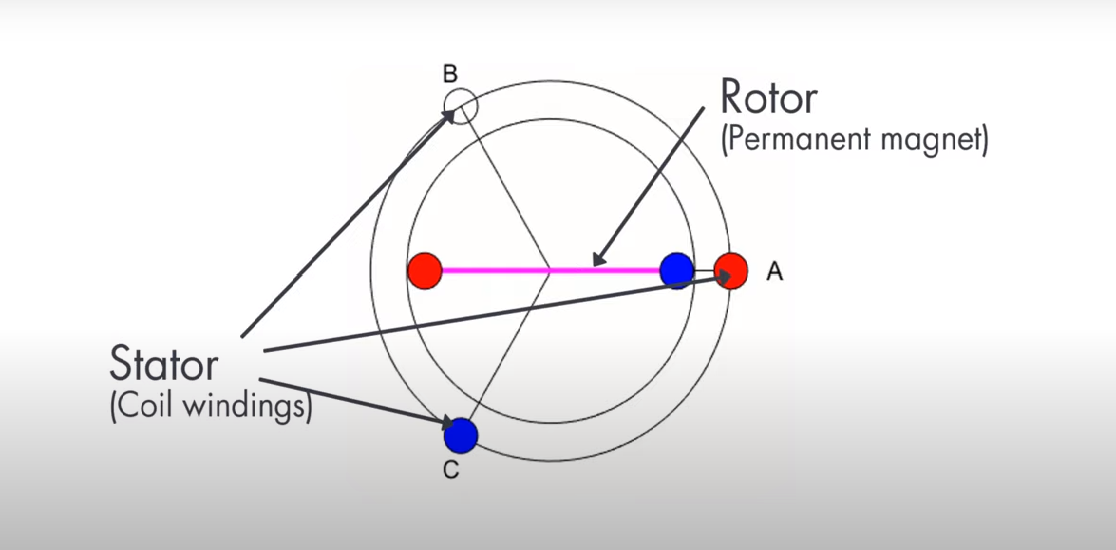
\includegraphics[scale=.5]{MOTOR STRUCTURE.png}}
\caption{Figure 1.1: Motor Structure}
\usepackage{}
\justifying

 This figure 1.1 shows the structure of bldc motor in which three phase coils 
\vspace{2cm}

\centering
\centerline{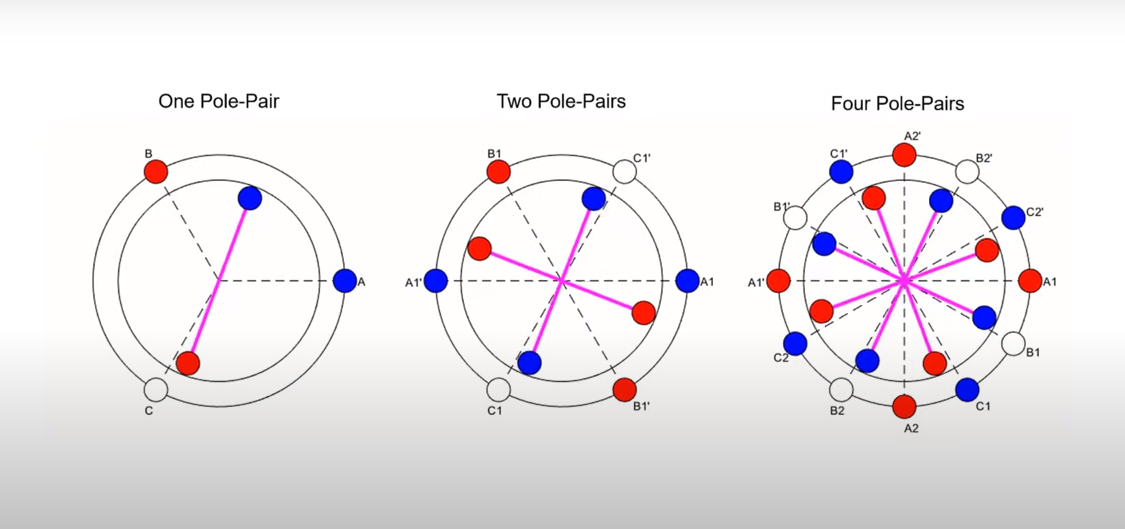
\includegraphics[scale=.5]{MOTOR STRUCTURE pp.png}}
\caption{Figure 1.2: Motor Structure With Different Pole pairs}
\vspace{2cm}
\\The Figure 1.2 shows the arrangement for different pole pairs configurations. 

\chapter{Literature Survey}
\usepackage{}
\justifying
AN885, Brushless DC (BLDC) Motor Fundamentals This paper explains about the basic fundamentals that includes its construction , working principle , torque speed characteris-tics and commutation sequence[1]. 




\chapter{Brushless Direct current Motor: Speed control  from various controllers }
In this section two different methods of speed control is studied to identify the best method to use. 

\section{PID Control}
The whole BLDC motor system is connected with the PID controller

 
\subsection{Data Collection}

\begin{tabular}{ |p{3cm}||p{3cm}|p{3cm}|p{3cm}|  }
\hline
\multicolumn{4}{|c|}{PID CONTROL PARAMETERS} \\
\hline
Parameter Name & Value & Min & Max\\
\hline
Kp  & 0.342  &0.342 &0.342 \\
Ki&  37.1910  &37.1910  &37.1910\\
Kd &50.000& 50.000& 50.000\\
\hline
\end{tabular}
\vspace{2cm}
\\This table shows values of different parameters of PID controllers.
\subsection{Results}
These are the Response Obtained after Simulations in which X axis serves as Time in seconds and Y axis serves as speed in Radians Per Second.

\begin{figure}[htbp]
\centerline{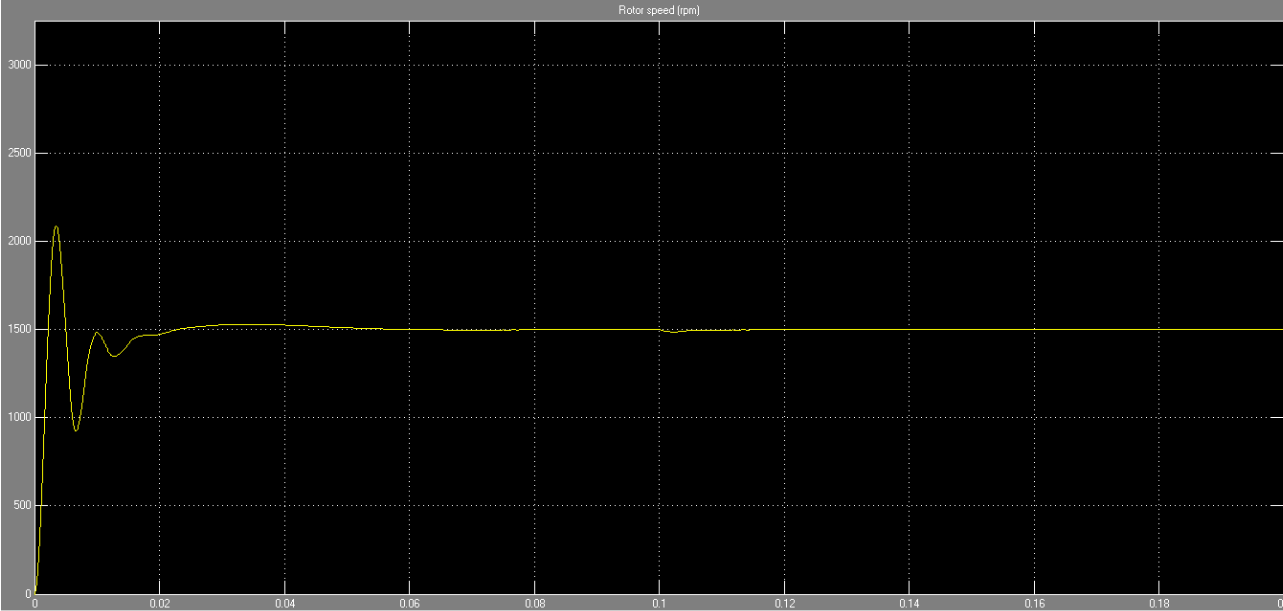
\includegraphics[width=\textwidth]{PID Good Quality photo.png}}
\caption{ PID Response of the Model }
\label{ddata}
\end{figure}









\section {PII Control} 
In this model the whole BLDC motor system is connected with the PII controller 


 \\
%\vspace{10cm}
\paragraph{Paramenters value} These are the values of different parameters 


\vspace{5cm}

%Main Building : 6814.02 m2\\


\begin{tabular}{ |p{3cm}||p{3cm}|p{3cm}|p{3cm}|  }
\hline
\multicolumn{4}{|c|}{PII CONTROL PARAMETERS} \\
\hline
Parameter Name & Value & Min & Max\\
\hline
Kp  & 0  &0&0\\
Ki&  50.000  & 50.000  &50.000\\
Kd &0.0036& 0.0036&  0.0036\\

\hline
\end{tabular}







\hspace{1cm}
\subsection{Results}
These are the Response Obtained after Simulations 





\chapter{Conclusions}
By measuring the performances of Brushless Direct Current Motor among PID and 


\newpage 


%\addtocontents{toc}{\protect\contentsline{chapter}{References}{}}


\cleardoublepage

\phantomsection
\renewcommand\bibname{References}
\addcontentsline{toc}{chapter}{References}

\begin{thebibliography}{9}

\bibitem{b1} Padmaraja Yedamale Microchip Technology Inc: Brushless DC (BLDC) Motor    Fundamentals . AN885 (2003)

\bibitem{b2} A. Purna  Chandra  Rao ,Y.P. Obulesh and Ch. Sai Babu :  MATHE-MATICAL MODELLING OF BLDC MOTOR WITH CLOSED LOOPSPEED CONTROL,USING PID CONTROLLER. ARPN Journal of Engineering and Applied Science. VOL. 7, NO. 10,( 2012) 

\bibitem{b3} Bilal Akin, Manish Bhardwaj : Trapezoidal Control of BLDC MotorsUsing Hall Effect     Sensors. TEXAS INSTRUMENTS,(2013)

\bibitem{b4}*Y.Narendra Kumar, ** P.Eswara Rao, **P. Vijay Varma, **V. V. RamVikas,  **P.  Kasi  Naidu  Speed  Control  of  Bldc  Motor  Drive  by  UsingPid Controllers.  Int. Journal of Engineering Research and Applications ISSN : 2248-9622, Vol. 4, Issue 4( Version 4),( 2014),  

\bibitem{b5} T. Govindaraj, V. Purushothaman : Simulation Modeling of Inverter Controlled BLDC Drive Using Four Switch. ijair.jctjournals.(2013) 

\bibitem{b6}6.	U. Neethu and V. R. Jisha, "Speed control of Brushless DC Motor: A comparative        study,"  IEEE International Conference on Power Electronics, Drives and Energy Systems (PEDES), 2012, pp. 1-5, doi: 10.1109/PEDES.2012.6484349.(2012)

\bibitem{b7}  S.Abraham: MODIFIED TIME SHARING SWITCHING TECHNIQUE FOR MULTIPLE  INPUT DC-DC CONVERTER FED PMDC DRIVE. @inproceedings
                 (2014)



\end{thebibliography}
\end{document}
